\section{Introduction to Fourier Analysis}
\noindent In the natural sciences, the procedure to search for periodic signals in datasets goes by various names, including spectral analysis, harmonic analysis or Fourier analysis. The latter name refers to Jean-Baptiste Joseph Fourier (1768 -- 1830), the French mathematician who was especially interested in heat transfer and vibrations (he is also generally credited for the discovery of the greenhouse effect). Using his considerable smarts, Fourier realized that any function $x(t)$, so long as it was single-valued (i.e., one value of $x(t)$ for every value of $t$), could be represented as the sum of a series of cosine waves taking this form:

\begin{align}
x_k(\theta) = A_k \mathrm{cos}(k\theta - \phi_k) \qquad
\end{align}

\noindent where $\theta$ is an angular variable for a function $x_k(\theta)$, with a period of $2\pi$ radians. Thus, for a given frequency $k$, the value $x(\theta)$ is determined by $A_k$ (the amplitude of the wave) and the phase angle $\phi_k$ (if $\phi_k$ = $\pi/2$ radians, or 90$^{\circ}$, then $\phi_k$ could be dropped and the cosine function replaced with the sine function). If we rely on the following trigonometric identity for difference between two angles, $R$ and $S$:

\begin{align}
\mathrm{cos}(R-S) = \mathrm{cos}(S)\mathrm{cos}(R) + \mathrm{sin}(S)\mathrm{sin}(R) \qquad
\end{align}

\noindent we can re-write equation 1 as:

\begin{align}
x(\theta) = A_k \mathrm{cos}(\phi_k)\mathrm{cos}(k\theta) +  A_k \mathrm{sin}(\phi_k) \mathrm{sin}(k\theta)\qquad
\end{align}

\noindent and because the phase angle is constant for a given frequency, we can define constants $a_k = A_k \mathrm{cos}(\phi_k)$ and $b_k =  A_k \mathrm{sin}(\phi_k)$, and the general formula for a cosine wave becomes:

\begin{align}
x_k(\theta) = a_k \mathrm{cos}(k\theta) +  b_k \mathrm{sin}(k\theta) \qquad 
\end{align}

\noindent a sum of both a cosine and a sine function. Returning to Fourier and his realization, we can now write a formula for the \textit{Fourier series}:

\begin{align}
x(\theta) &= \frac{a_0}{2} + \sum_{k=1}^{\infty} a_k \mathrm{cos}(k\theta) + \sum_{k=1}^{\infty} b_k \mathrm{sin}(k\theta) \qquad \\
\end{align}

\noindent where we have simplified for the case when k = 0. This series means that  any $x(t)$ could be expressed this way, where $x(t)$ = $x(\theta)$. At this point, it is helpful to express $\theta$ as a function of $t$, our original independent variable, and $T$, the duration of $x(t)$, which is set to the period of the sinusoid, $2\pi$. Hence, the first non-zero frequency in our Fourier series (also called the \emph{fundamental} or \emph{first harmonic} frequency) is $f_1$ = $1/T$. All the other non-zero-frequencies in a Fourier series are harmonics (integer multiples) of this fundamental frequency, i.e. the second harmonic is $f_2$ = $f_1$ + $\Delta$f = 2$f_1$, third harmonic is  $f_3$ = $f_2$ + $\Delta$f = 3$f_1$. Thus, the $k^{th}$ frequency in our summation is $f_k$ = $f_{k-1}$ + $\Delta$f = k$f_1$. This enables us to write the general form for the Fourier series of a time function $x(t)$ of period $T$:

\begin{align}
x(t) &= \frac{a_0}{2} + \sum_{k=1}^{\infty} a_k \mathrm{cos}(\frac{2\pi k}{T}t) + \sum_{k=1}^{\infty} b_k \mathrm{sin}(\frac{2\pi k}{T}t) \\
x(t) &= \frac{a_0}{2} + \sum_{k=1}^{\infty} a_k \mathrm{cos}(2\pi f_k t) + \sum_{k=1}^{\infty} b_k \mathrm{sin}(2\pi f_k t) \qquad 
\end{align}

\noindent If we next rely on Euler's formulas:

\begin{align}
e^{i\theta} &= \mathrm{cos}(\theta) + i \mathrm{sin}(\theta) \\
e^{-i\theta} &= \mathrm{cos}(\theta) - i \mathrm{sin}(\theta) \qquad 
\end{align}

\noindent where $e$ is Euler's number ($e = 2.718281828459 .... $) and $i$ is the imaginary number $i = \sqrt{-1}$. If one does enough algebra and trigonometry, one can rewrite Equation 8 as a \textit{complex Fourier series}:

\begin{align}
x(t) =  \sum_{k=-\infty}^{\infty} c_k e^{2\pi i f_k t} \qquad 
\end{align}

\noindent The complex coefficients $c_k$ tell you the required \emph{amplitude} of the cosine and sine waves for each frequency $f_k$ needed to reproduce $x(t)$. They relate directly to the real coefficients $a_k$ and $b_k$ according to the following formulas:

\begin{align}
c_k &= \frac{1}{2}(a_k - i b_k)\\
c_k &= \frac{1}{T} \int_{0}^{T}x(t) (\mathrm{cos} (2 \pi f_k t) - i \mathrm{sin} (2 \pi f_k t)) dt\\
c_k &= \frac{1}{T} \int_{0}^{T}x(t) e^{-2\pi i f_k t} dt
\end{align}

\begin{figure}[ht]
	\centering
	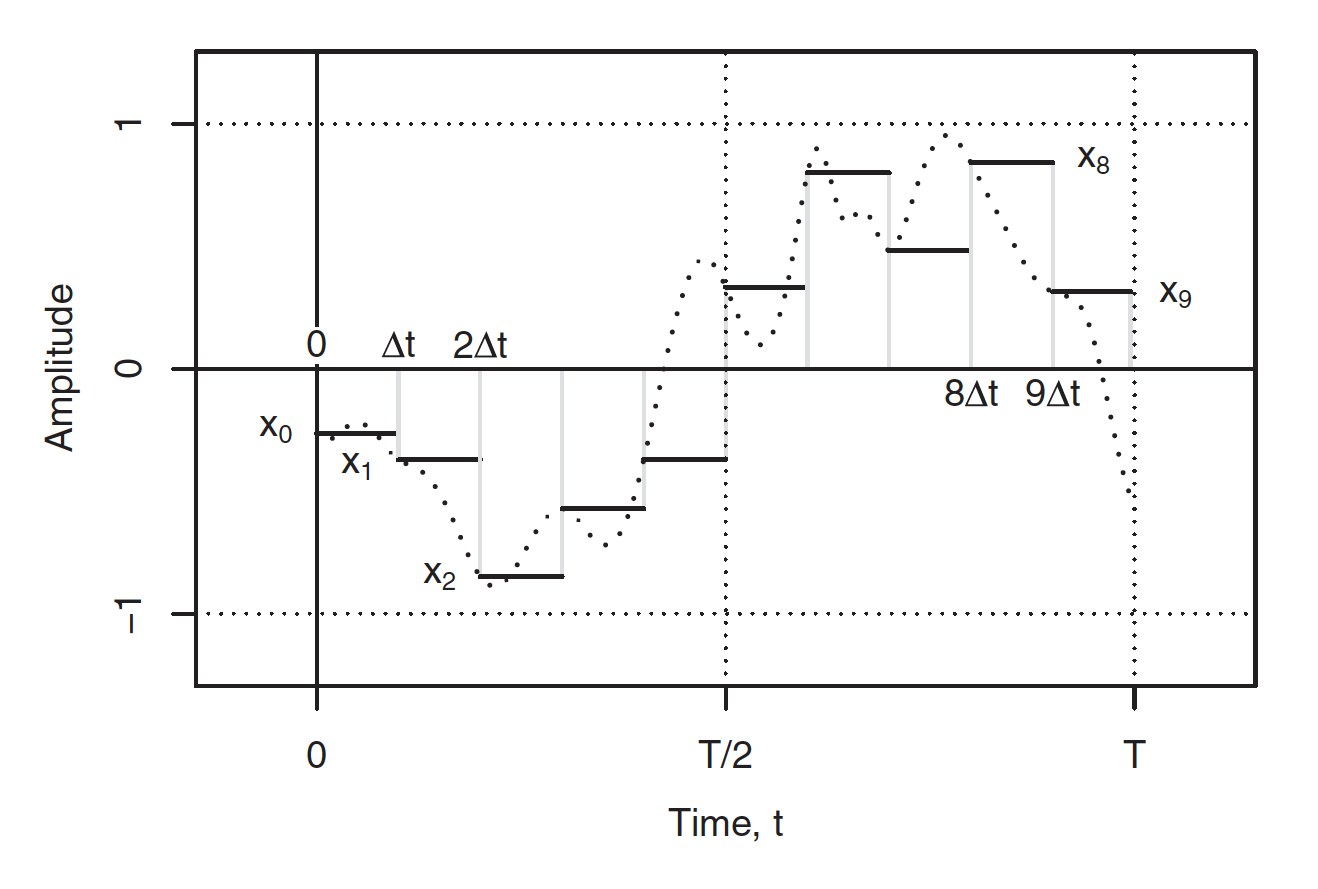
\includegraphics[width=1\textwidth]{figures/discrete_function.png} % requires the graphicx package
	\caption{a discrete approximation of a continuous function}
		\label{fig:discrete}
\end{figure}


\section{Discrete Fourier Transform}

Of course, while mathematicians can deal with functions or time series that stretch to infinity, scientists are always dealing with finite numbers (Fig.~\ref{fig:discrete}). Measurements taken from a stratigraphic section, for example, have a beginning and an end (covering some period $T$). The dataset will consist of a series of values (numbered $n_0$, $n_1$, $n_2$, etc.), making up some total number of samples ($N$). Each sample is separated by a \emph{sampling interval} ($dt$, assumed here to be equal - \emph{this is very important!}). Any resulting time series or stratigraphic series ($x_n$) is always going to be a discrete approximation of some continuous function ($x(t)$, representing, for example, changing sea level with time.
\\

\noindent Thus, we need an approach for describing the sinusoids needed to describe a \emph{discretized} time series, $x_n$ (Fig.~\ref{fig:discrete}). In other words, we need a discrete version of equation of Equation 14, and this equation takes this form:

\begin{align}
X_k &= \frac{1}{N} \sum_{n=0}^{N-1}x_n e^{-2\pi i \frac{kn}{N}} \qquad 
\end{align}

\noindent where $X_k$ is being used in place of $c_k$ (but is otherwise the same as $c_k$). Equation 15 is the basic forward discrete Fourier transform. The index $k$ (frequency) also ranges between $0\leq k \leq N-1$, like $n$ (time). Thus, equation 15 is really a system of linear equations:

\begin{align}
\mathbf{\underline{X}} = \begin{pmatrix} X_0 \\
			      X_1\\ 
			      .\\
			      .\\
			      .\\
			      X_k\\
			      .\\
			      .\\
			      .\\
			      X_{N-1}\\
       \end{pmatrix}
      ~\mathrm{and}~
      \mathbf{\underline{x}} = \begin{pmatrix} x_0 \\
			      x_1\\ 
			      .\\
			      .\\
			      .\\
			      x_n\\
			      .\\
			      .\\
			      .\\
			      x_{N-1}\\
       \end{pmatrix} \qquad 
\end{align}

\noindent with Equation 15 becoming:

\begin{equation*}
\mathbf{\underline{X}} = \mathbf{F}\mathbf{\underline{x}}
\end{equation*}

\noindent and performing a \emph{fast Fourier transform} solves it through matrix algebra, the lowest frequency resolved is $1/T$, where $T$ is the total time represented by the time series (also equal to $N \cdot dt$). If $N$ (the number of data points) is even, the highest resolved is frequency 1/(2$dt$), where $dt$ is the sampling interval. In between these two end-points, each resolved frequency is separated by $1/T$. With these FFT coefficients ($X_k$), which again tell you the \emph{amplitude} of each cosine and sine wave for each frequency $k$, one can always exactly recreate the original time series $x_n$.

\begin{figure}[b!]
	\centering
	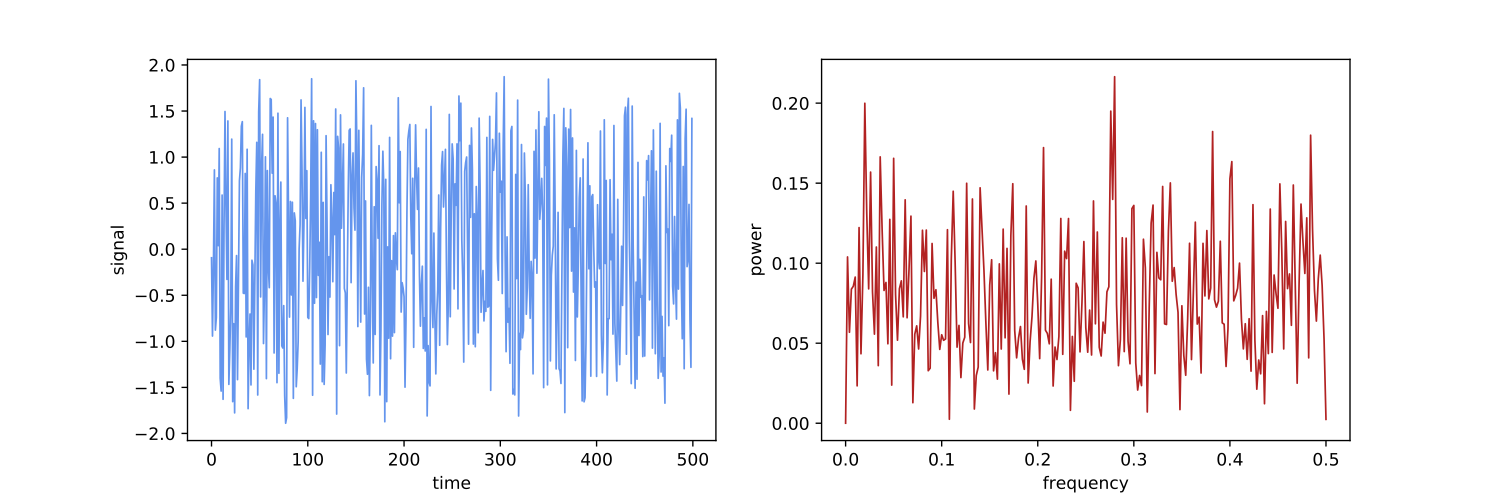
\includegraphics[width=1\textwidth]{figures/white_noise.png} % requires the graphicx package
	\caption{A time series $x_n$ made of white noise (left), and the fast Fourier transform ($X_k$) on the right. The y-axis of the FFT indicates the relative contribution of each sinusoid frequency in explaining the total signal, and can be used to exactly reproduce the original blue curve. }
		\label{fig:noise}
\end{figure}

\noindent When doing Fourier analysis with the aim of identifying periodic signals, it is important to remember this fact: \emph{any time series can be described as a summation of periodic signals}, including pure white noise (Fig.~\ref{fig:noise}). If you have 100 data points that you think records sea level change over the last 100 years, and you discover that it can be perfectly described by 50 sinusoids, you have not discovered that sea level has 50 nested cycles - you have simply demonstrated the Fourier relationship (Equation 1). Instead, what we are looking for with such an analysis is: does a periodic signal explain a significant amount of the variation within a time series? If a significant peak is located, does this periodic signal \emph{make sense} as a potential driver of Earth system change (i.e., is it a known or expected frequency of change in climate, etc.)? Keep these concepts in mind as you explore two different datasets below!
